\documentclass[10pt,twocolumn]{article}

\usepackage{isqcmc2023}
\usepackage{graphicx,hyperref}
\usepackage{subcaption}

%\usepackage[brazil]{babel}
%\usepackage[latin1]{inputenc}
% If needed, change this to:
\usepackage[utf8]{inputenc}

\sloppy

\title{Sonifying Quantum Superpositions by Correlating State Probability to Rhythmic Density}

\author{Walker Smith\inst{1} \and
        Dmitri Volkov\inst{1} \and
        Alex Alani\inst{1}}

\address{Jacobs School of Music -- Indiana University Bloomington\\
         107 S. Indiana Ave. - 47405 - Bloomington - Indiana - United States of America
         \email{walksmit@iu.edu, dvolkov@iu.edu, alealani@iu.edu}
}

\begin{document}

\maketitle

\begin{abstract}
In this paper we introduce a novel approach for sonifying a superposition of quantum states, by using rhythmic density (e.g. faster rhythms) to represent probability amplitudes. Typical sonifications of quantum superpositions assign a different musical pitch to each state and correlate the probability of each state to the respective pitch’s loudness. However, this has problems of quantifiability, which our novel approach rectifies. With our sonification methods, we hope to help listeners obtain an intuitive understanding of the probabilitistic nature of quantum systems. Herein we present an overview of our approach and a discussion of how it compares to prior work and other quantum sonification methods. We discuss the advantages and disavantages of our work and conclude by outlining areas for future development and research.
\end{abstract}

\section{Introduction}

Quantum computation is an emerging field with many promising applications across a wide variety of disciplines\cite{ukpabi2023framework}. However, it is often tricky to gain an intuitive understanding of how quantum computation (and quantum systems in general) work in practice\cite{qcvc}. That said, music has a rich history of explaining difficult concepts in intuitive ways \cite{watzke2022}\cite{smith2022}, dating back at least as far as Johannes Kepler\cite{rodgers1979}. By aligning unintuitive concepts of quantum computation with intuitive concepts in music, we hope to enable a wider audience to understand the underpinnings of quantum computation, as well as give experienced quantum practitioners a new tool for analysis. In this paper, we introduce a new paradigm for sonification of quantum systems by correlating higher amplitudes of a state with greater rhythmic density (e.g. faster rhythms).

\subsection{Quantum Superposition}

Arguably, the primary difference between classical information and quantum information is that quantum information can exist in superposition. As such, we choose to focus on sonifying superpositions of quantum states. By focusing on superpositions, we provide a solid bedrock for future work (briefly explored at the end of the paper) for sonifying other aspects of a quantum system, including entanglement and phase.

\subsection{Rhythmic Density and Probability}

Our approach to sonifying a quantum state is as follows: first, calculate the probability of measurement for each of the basis states, then use these probabilities as input to one of several rhythmic density based sonification algorithms. These sonification algorithms map a higher probability to higher rhythmic density with faster rhythms and more notes, while lower probabilities correlate to lower rhythmic density with slower rhythms and less notes. As we outline later in the paper, rhythmic density is highly quantifiable for the human ear compared to other potential “sonification dimensions,” and has other advantages as well. While our approach is infeasible to run on quantum hardware (because a useful approximation of the probabilities of a quantum state on hardware requires many invocations of the same program), it is still very useful with smaller simulated quantum systems as a pedagogical tool, analytical too, and creative tool for musicians.

\section{Prior Work}

\subsection{qMuVi}

Several effective sonification models have been applied to representation of quantum computers. The qMuVi\cite{qmuvi} project, developed by researchers at the University of Melbourne, sonifies quantum states in N-qubit systems by assigning each of the 2N states to a unique pitch. For example, a 2-qubit system with the 4 measurement basis states $\{|00\rangle, |01\rangle, |10\rangle, |11\rangle\}$ can be represented by 4 distinct, arbitrary pitches. A superposition of multiple states thus sounds like a chord with multiple notes, where the loudness of each note is related to its probability.

This is an intuitive musical mapping, but it suffers from a problem of quantitative representation of the respective probabilities (as outlined in section \ref{sec:Why Rhythmic Density}). Additionally, discerning loudness differences in superimposed tones can be difficult, especially if those tones are far apart in frequency-space, due to the uneven perception of loudness across the frequency spectrum\cite{smyth2019} We propose that correlating probability to rhythmic density instead of loudness will more accurately represent the quantitative relationships between probability values in a superposition state.

\subsection{Q1Synth}

Another approach to sonifying a qubit is demonstrated by the Q1Synth\cite{q1synth}, developed by the ICCMR at University of Plymouth. Besides sonification, the Q1Synth also provides visualization of a qubit in the form of a Bloch sphere, which shows the amplitudes and phases as a position on a three-dimensional sphere. The point on the top of the sphere represents the $|0\rangle$ state, and the point on the bottom represents the $|1\rangle$ state; points in the middle represent linear combinations of the two states, with a phase indicated by where along the sphere they lie. The general sonification approach of the Q1Synth is to take the polar coordinates of the position of the point of the Bloch sphere and use these as parameters for one of several synthesis methods, including FM synthesis, additive synthesis, and granular synthesis.

Q1Synth presents two ways for users to interact: by freely rotating the Bloch sphere using a mouse or other input device and activating a measurement operator which collapses the qubit represented by the Bloch sphere into either a $|0\rangle$ or $|1\rangle$ state. When the measurement occurs, a circuit is constructed which assembles a state identical to that represented by the Bloch sphere and runs this circuit on quantum hardware to figure out how the collapse occurs.

Besides being an effective use of quantum hardware for live settings, Q1Synth is a powerful creative tool, and useful for understanding how measurement affects a quantum system. That said, its utility as a pedagogical and analytical tool is limited in some ways. Firstly, by choosing to use a Bloch sphere as the primary representation of a qubit, it is limited to sonifying only single-qubit systems. While it is possible to have multiple instances of Q1Synth running in parallel, with the current implementation they cannot entangle or otherwise interfere with each other, as might be the case for many composite quantum systems. Secondly, the interaction mechanism of freely rotating a Bloch sphere is misrepresentative of how qubits tend to be interacted with in practice; instead of specifying a quantum state and having a circuit or other transformation system generated after, most quantum systems take the form of applying transformations to one state and getting another as a result\cite{qmdistilled}. As such, Q1Synth’s ability to sonify existing quantum systems is limited.

Our work counters these issues by generalizing to any number of quantum states, whether they are states of a qubit-based system or of any other type of quantum system. Furthermore, our work sonifies existing sequences of quantum state transformations, and so can be applied to nearly any existing quantum system. That said, our mechanism requires a quantum simulation, so there is an upper limit to the size of the system that we can sonify.

\section{Why Rhythmic Density} \label{sec:Why Rhythmic Density}

Rhythmic density here refers to how many notes occur within a uniform span of time. For example, a span of a second with 5 notes has greater rhythmic density than a span of a second with a single note. Note that this definition holds even if the note durations within the span are not the same. To differentiate between different basis states, each state is assigned a different pitch and/or timbre.

To achieve a more quantitative representation of the probabilities of states, we correlate the probabilities of each quantum state with higher rhythmic density for the pitch/timbre assigned to each state. According to our paradigm, a pitch corresponding to a state with a higher probability of being measured will produce more attacks in a unit of time than a pitch corresponding to a state with a lower probability. In other words, measurement probability is positively correlated with rhythmic density.

For example, consider a single qubit in an equal superposition state, $|+\rangle = \sqrt{\frac{1}{2}}|0\rangle + \sqrt{\frac{1}{2}}|1\rangle$. Here, the measurement probabilities of $|0\rangle$ and $|1\rangle$ are both $\frac{1}{2}$, so they are the same. Because both measurement probabilities are the same, both states should have the same rhythmic density. With our sonification method, each state is assigned to an arbitrary pitch (say C4 and G4 for |0> and |1>, respectively), and the rhythms corresponding to both states would be the same (Figure \ref{fig:Figure1a}).

On the other hand, consider the state $\sqrt{\frac{1}{4}}|0\rangle + \sqrt{\frac{3}{4}}|1\rangle$. Here, the probability of measurement for the $|0\rangle$ state is $\frac{1}{4}$, and the probability of measurement for the $|1\rangle$ state is $\frac{3}{4}$. So the $|1\rangle$ state is three times as likely as the $|0\rangle$ state to be measured, and thus should have three times the rhythmic density.  As such, the ratio of the rhythms corresponding to the $|0\rangle$ and $|1\rangle$ states would be $1:3$ (Figure \ref{fig:Figure1b}).

\begin{figure}[h]

        \begin{subfigure}{0.45\textwidth}
                \centering
                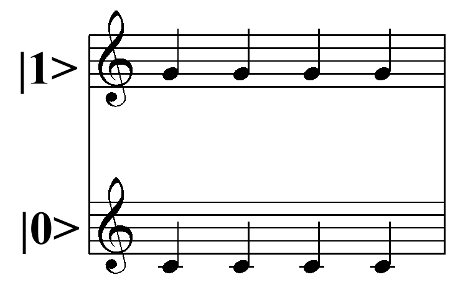
\includegraphics[width=\textwidth]{fig/Figure 1a.png} % first figure itself
                \caption{Rhythm-based sonification of a superposition of $\sqrt{\frac{1}{2}}|0\rangle + \sqrt{\frac{1}{2}}|1\rangle$, where the measurement probabilities of $|0\rangle$ and $|1\rangle$ are equal, so the corresponding rhythmic density of C4 and G4 are equal.}
                \label{fig:Figure1a}
        \end{subfigure}

        \hfill

        \begin{subfigure}{0.45\textwidth}
                \centering
                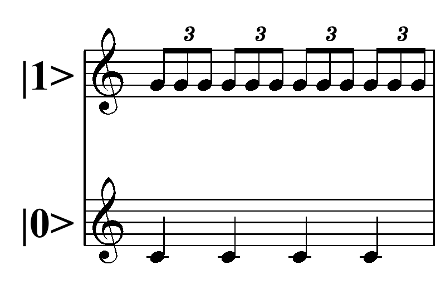
\includegraphics[width=\textwidth]{fig/Figure 1b.png} % second figure itself
                \caption{Rhythm-based sonification of a superposition of $\sqrt{\frac{1}{4}}|0\rangle + \sqrt{\frac{3}{4}}|1\rangle$, where the measurement probabilities of $|0\rangle$ and $|1\rangle$ are $\frac{1}{4}$ and $\frac{3}{4}$, respectively. Thus, the corresponding rhythmic density of G4 ($|1\rangle$) is three times that of C4 ($|0\rangle$).}
                \label{fig:Figure1b}
        \end{subfigure}

        \caption{}
        \label{fig:Figure1}

\end{figure}

\subsection{Rhythmic Density vs. Loudness}

Existing approaches to sonifying superposition have used loudness to represent a higher measurement probability\cite{qmuvi}. While this is intuitive in the sense that it directly maps probability amplitudes with sound wave amplitudes, in reality it is difficult for the human ear to recognize precise differences in loudness\cite{kulkarni2001}.

To hear an audio representation of this principle and understand the difficulty of discerning quantitative amplitude relationships of sound waves, consider audio excerpts 1-3\footnote{Audio excerpt 1: \url{https://drive.google.com/file/d/1QB20vdteN57-Er__1ZCr1-wYSQJh6fRT} \\ Audio excerpt 2: \url{https://drive.google.com/file/d/1DvcFW1d_TErt6XYo23-TAbJp4Uyr48S0} \\ Audio excerpt 3: \url{https://drive.google.com/file/d/197T5tmc66V7h7W4tXEX2yas0zRbZJ-Ek}}.
Each excerpt is a conventional (i.e. correlating probability with loudness) sonification of a qubit in a unique superposition of: $\sqrt{x}|0\rangle + \sqrt{y}|1\rangle$, with two sine tones with frequencies corresponding to C5 and E5 for $|0\rangle$ and $|1\rangle$, respectively. The ratio of loudness C5/E5 is determined by the ratio x/y. The reader is encouraged to listen to each audio excerpt and, from the loudness of each tone, predict the approximate values of x and y. In other words, try to identify the louder tone (if any), and how much louder one tone is than the other.

We expect the reader to find this to be a challenging task. Even if one could identify the louder tone, it is very difficult to tell how much louder it is. Now let’s consider our method which correlates the probability to rhythm. Audio excerpts 4-6\footnote{Audio excerpt 4: \url{https://drive.google.com/file/d/13kcnMuCuH-ELfUf8wU_LtiU61ROKRqT9} \\ Audio excerpt 5: \url{https://drive.google.com/file/d/1MT6_Z_2fvYsoN6l_w5m2s_1etNm2U8Mn} \\ Audio excerpt 6: \url{https://drive.google.com/file/d/14PxUmYv_vjKKM7ldgCbZMRo8hJ5CXvwn}} represent the same three superpositions with the same three probability amplitudes, but this time the ratio of x/y is sonified as rhythmic density. The tones are not constant but rather repeat at specific time intervals, and the rate of repetition is determined by the probability ratio x/y. Now, try to approximate the ratio x/y for each superposition. In other words, try to identify which note is being repeated faster (if any), and how many times faster that note is being repeated. This exercise will be familiar to music students forced to do rhythmic dictation in ear-training classes.

Even without having had the pleasure of taking an ear-training course, it is likely easier to identify the relative probabilities in excerpts 4-6 than in 1-3. The easily quantifiable nature of rhythmic values and note-length-relations compares favorably to the extreme difficulty of comparing loudness. Notating audio excerpts 4-6 in standard musical staff notation makes this clearer (Figure \ref{fig:Figure2}).

\begin{figure}[h]

        \begin{subfigure}{0.45\textwidth}
                \centering
                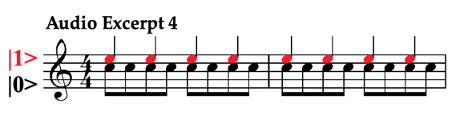
\includegraphics[width=\textwidth]{fig/Figure 2a.png} % first figure itself
        \end{subfigure}

        \hfill

        \begin{subfigure}{0.45\textwidth}
                \centering
                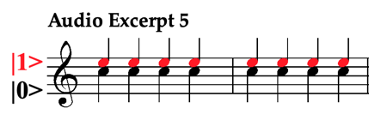
\includegraphics[width=\textwidth]{fig/Figure 2b.png} % second figure itself
        \end{subfigure}

        \begin{subfigure}{0.45\textwidth}
                \centering
                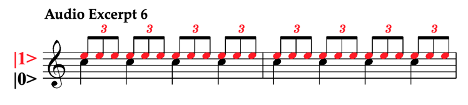
\includegraphics[width=\textwidth]{fig/Figure 2c.png}
        \end{subfigure}

        \caption{Score notations for audio excerpts 4, 5, and 6. From this it is clear that the probability ratios of $|1\rangle$ to $|0\rangle$ in each excerpt are $1:2$, $1:1$, and $3:1$, for excerpts 4, 5, and 6, respectively.}
        \label{fig:Figure2}
\end{figure}

Consider a more complicated example: a two-qubit system in a superposition of $\sqrt{x_1}|00\rangle + \sqrt{x_2}|01\rangle + \sqrt{x_3}|10\rangle + \sqrt{x_4}|11\rangle$, with $x_1:x_2:x_3:x_4$ equal to $1:2:3:4$. In other words, a superposition defined by $\sqrt{\frac{1}{8}}|00\rangle + \sqrt{\frac{1}{4}}|01\rangle + \sqrt{\frac{3}{8}}|10\rangle, \sqrt{\frac{1}{2}}|11\rangle$. We can arbitrarily assign the pitches C5, E5, G5, and Bb5 to the states $|00\rangle$, $|01\rangle$, $|10\rangle$, and $|11\rangle$, respectively.

Audio excerpt 7\footnote{Audio excerpt 7: \url{https://drive.google.com/file/d/1c5eaA8SZ9PbVJj77imOpTU4KQXowH388}} provides a realization of this rhythmic result, and Figure \ref{fig:Figure3} provides a score notation.

\begin{figure}[h]
\centering
  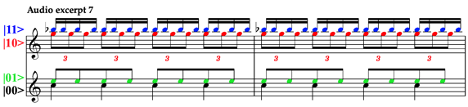
\includegraphics[width=.45\textwidth]{fig/Figure 3.png}
\caption{Score notation for audio excerpt 7, where the probability ratio of $|11\rangle : |10\rangle : |01\rangle : |00\rangle$ can be heard as $4:3:2:1$}
\label{fig:Figure3}
\end{figure}

Discerning the rhythmic relationships is certainly more challenging here, but for a loudness-based approach it would be virtually impossible. Audio excerpt 8\footnote{Audio excerpt 8: \url{https://drive.google.com/file/d/1XWeXW7VmTLlRR7t9RMDjlbJSXT1gcNmU}} provides such a realization, and it is immediately clear that it is difficult to even rank the loudness of all 4 pitches, let alone determine the precise loudness relationships.

Additionally, the four pitches can be separated further in pitch space to make it easier to distinguish each state. Audio excerpt 9\footnote{Audio excerpt 9: \url{https://drive.google.com/file/d/1bS-znqhmzAkNA4vvftrIKMgVT0wVOjh6}} and Figure \ref{fig:Figure4} show the same sonification as audio excerpt 7 (Figure \ref{fig:Figure3}), but with certain notes displaced by one or more octaves. The pitch-class associated to each state is still the same (C: $|00\rangle$, E: $|01\rangle$, G: $|10\rangle$, Bb: $|11\rangle$), although the notes are displaced to different octaves (C2: $|00\rangle$, E3: $|01\rangle$, G4: $|10\rangle$, Bb5: $|11\rangle$), instead of all being in the same octave as C5.

\begin{figure}[h]
\centering
  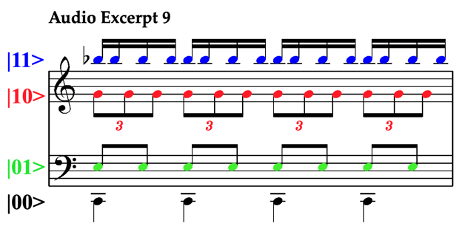
\includegraphics[width=.45\textwidth]{fig/Figure 4.png}
        \caption{Score notation for audio excerpt 9, the same sonification as audio excerpt 8 (Figure \ref{fig:Figure3}) with C, E, G, and Bb displaced by -3, -2, -1, and 0 octaves, respectively.}
\label{fig:Figure4}
\end{figure}

While the probability ratios chosen for the above examples are admittedly contrived in order to result in easily-notated score excerpts, this method can of course be applied to any probability ratios, and is applied to simulations of quantum circuits in section \ref{sec:Implementations}.

\subsection{Assigning a Unique Instrument (Timbre) to Each State}

For our approach to be useful in more complicated systems, we not only adopt this probability-rhythmic density idea, but also represent each state with a unique instrument. Thus, the combination of instrument and pitch is unique for every state. In this case, instrument refers abstractly to the pitch being played with a unique timbre, and thus may imply acoustic instruments or different electronic waveforms. Audio excerpt 10\footnote{Audio excerpt 10: \url{https://drive.google.com/file/d/15OuTjLkb0Wk7XkEk6S0yqA2Iwyhfm73A}} is the same as audio excerpt 7, except each state has been assigned to a different instrument (Figure \ref{fig:Figure5}).

\begin{figure}[h]
\centering
  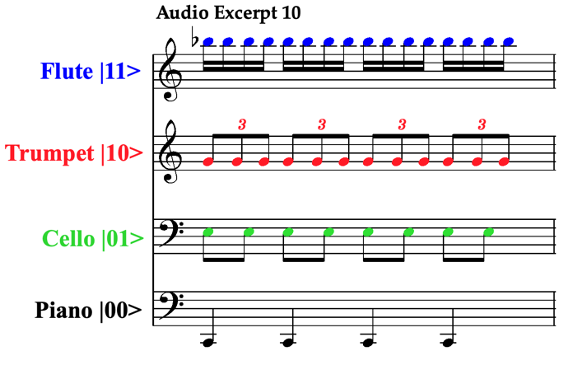
\includegraphics[width=.45\textwidth]{fig/Figure 5.png}
        \caption{Assigning a different instrument and pitch to each state.}
\label{fig:Figure5}
\end{figure}

By assigning each state to a unique instrument in different, non-overlapping frequency ranges, frequency masking (e.g. when one sound makes it hard to hear another because the frequencies overlap) is unlikely to occur, making it easy to tell the instruments apart\cite{smyth2019}. Choosing instruments with easily distinguishable timbres also makes it easier to identify each state. In audio excerpt 10/Figure \ref{fig:Figure5}, the four instruments chosen represent different orchestral families with distinct timbres (woodwinds, brass, strings, piano). 

\subsection{Assigning a Unique Motive to Each State}

By assigning each instrument a pitch space instead of a single pitch, we unlock the option to use musical motives or lines instead of just single notes repeated with different rhythms. The motives (or motifs, as the two terms are often used interchangeably) are separated in pitch space, and have their own melodic contour. For example, a different motive can be assigned to each state, with the speed at which each motive is performed corresponding to the measurement probability. Figure \ref{fig:Figure6} shows a score notation assigning a different motive, instrument, and pitch-space to each of four states ($|00\rangle$, $|01\rangle$, $|10\rangle$, $|11\rangle$), and audio excerpt 11\footnote{Audio excerpt 11: \url{https://drive.google.com/file/d/1pWsGyKHENlIqA3gQ0BEH_1gWuMckoHDL}} plays these motives together. The motives chosen here combine to form a Bach-style chorale, but of course motives reflective of any genre/style could be chosen.

\begin{figure}[h]
\centering
  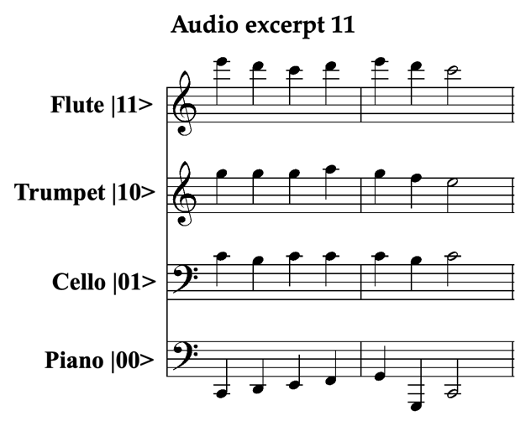
\includegraphics[width=.45\textwidth]{fig/Figure 6.png}
        \caption{Assigning a unique motive, instrument, and pitch-space to each state.}
\label{fig:Figure6}
\end{figure}

Now, different probability distributions will result in the entire motive being played faster or slower. Additionally, if certain states have zero probability, they will not sound at all and thus can be identified as absent from the musical texture. Figure \ref{fig:Figure6} (audio excerpt 11) shows all of these states in a $1:1:1:1$ probability ratio, but Figure \ref{fig:Figure7} (audio excerpt 12\footnote{Audio excerpt 12: \url{https://drive.google.com/file/d/1Af7gIBvu__nhb84qn640_obwTZ_uDy50}}) shows a ratio of probabilities of $1:2:0:1$ for $|00\rangle : |01\rangle : |10\rangle : |11\rangle$.

\begin{figure}[h]
\centering
  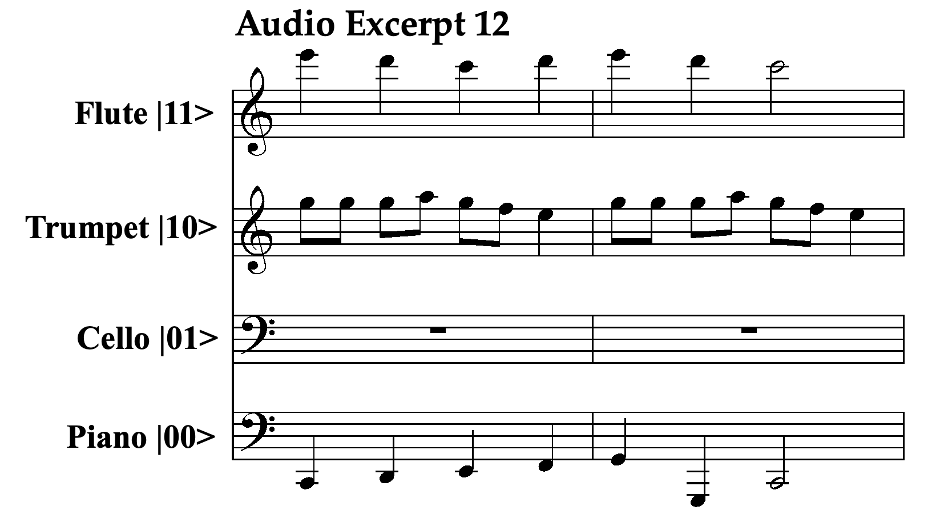
\includegraphics[width=.45\textwidth]{fig/Figure 7.png}
        \caption{Sonification of $|00\rangle : |01\rangle : |10\rangle : |11\rangle$ in $1:2:0:1$ probability ratio, with each state assigned to a distinct motive. The trumpet ($|10\rangle$) motive is played twice as fast as the flute and piano motives, as the probability of state $|10\rangle$ is twice as great as that of $|00\rangle$ (piano) and $|11\rangle$ (flute)}
\label{fig:Figure7}
\end{figure}

We view the utility of this method not necessarily as a pure sonification tool, but as a tool for 
algorithmic composition based on probabilities, as users can create motives and create musical textures and compositions algorithmically from the probabilities of superposition states. This shows that our methods can be applied to creative tasks in addition to creating auditory representations of superpositions.

\section{Implementations} \label{sec:Implementations}

To sonify a quantum circuit, we first need to extract parameters from it which we then can translate into sound. Due to the nature of quantum physics, it is not possible to extract information from a quantum system without disturbing it; furthermore, because a quantum system collapses upon measurement, some information is lost. For this reason, we chose to use a simulated quantum system through (Qiskit\cite{qiskit} and MicroQiskit\cite{microqiskit} though Max\cite{maxmsp}).While it technically is possible to adapt our method to run on quantum hardware, it would be computationally expensive, especially if one wants to hear how the state changes as it progresses through state transformations. As mentioned, it would require a large number of shots (e.g. quantum program invocations) to find a good approximation of the quantum state at a single stage\cite{qiskitalgos}. If one wanted to sonify the state as it progresses through state transformations, it would be necessary to perform the same number of shots at each stage in the computation, which would multiply the number of necessary shots. Furthermore, if the program being sonified itself requires a measurement operator, postselection would be necessary.

By using a simulated quantum computer, it becomes possible to accurately extract the statevector at each step in a quantum computation without disturbing the system\cite{qiskitstatevectordocs}. This gives us the probability amplitude for each quantum basis state. From this, we can calculate the probability of the measurement of each basis state by multiplying each probability amplitude by its complex conjugate. This gives us a single real number for each state, which we can feed into our sonification algorithms. While we do lose information about the phase, we can consider this as a separate parameter for each state. The sonification algorithms then generate note data, which then can be processed into sound data which is the final sonification.

\subsection{Python Implementation}

One implementation of this technique uses Python\cite{pythonlang} and the Qiskit\cite{qiskit} framework for working with quantum computers. We define a function, get\_probabilities\_at\_steps, which takes a user-defined Qiskit QuantumCircuit object and returns a list which has the statevector of the quantum system after each gate in the quantum circuit defined by the QuantumCircuit object. The implementation of this function simply iterates through the instructions from the user-provided QuantumCircuit and applies them to a fresh QuantumCircuit, using a Qiskit builtin to get the statevector of the fresh QuantumCircuit at each step. Another Qiskit builtin is then used to calculate the measurement probabilities for each basis state for each statevector.

The sonification approach used by our Python implementation transforms each probability into a rhythm by figuring out the ratio of each probability to the lowest probability, and giving each state a rhythm based on this ratio. This results in a polyrhythm between the notes, with ratios corresponding to the probabilities. 

The Python implementation is freely available via Google Colab\cite{googlecolab}. To use it, simply run the code blocks in order. This installs the necessary dependencies, defines helper functions, generates the circuit, and outputs a MIDI\cite{midi1spec} file for the sonified circuit! The MIDI data can then be processed into audio data by a digital audio workstation, such as Logic Pro\cite{logicpro} or Bitwig Studio\cite{bitwigstudio}. The circuit can be tweaked freely, using standard Qiskit conventions, in the 3rd code block. To download the MIDI file updated for the tweaked circuit, simply re-run the 4th code block.

The implementation can be accessed at the following link: \url{https://colab.research.google.com/drive/1Es9EgHPlMFIzgL5aJfddSCUdq9vngosS?usp=sharing} .

\subsection{Max Implementation}

The Max implementation is built atop the QAC Toolkit\cite{Hamido_2022} package, which in turn is built atop MicroQiskit\cite{microqiskit}. A circuit is defined in real-time by sending messages to an och.microqiskit object. Each message corresponds to the application of a quantum gate. We then use another message to extract the statevector. We send the statevector, along with the index of the desired state, to subpatchers which extract the corresponding probability amplitude for each state and convert them into probabilities. The outputs of each of these subpatchers can then be used as the input for a sonification method. Note that the circuit and subpatchers are constructed such that when any new gate is applied, the information propagates immediately through the system, without requiring any additional messages.

To use the Max implementation, download and open the Max file. Define messages which feed into the och.microqiskit object to perform the desired gates and operations on the quantum circuit. When ready to run, lock the circuit and press the box corresponding to each message to apply its operation to the quantum circuit. The sonification should update accordingly in real-time with each message sent!

\section{Limitations and Future Work}

\subsection{Evaluating Our Approach}

Our approach relies on the idea that rhythm-based sonification methods allow a listener to more easily determine the quantitative relationships between probabilities of states in a quantum superposition. However, this method would need to be evaluated alongside the traditional probability-loudness method with focus groups (ideally of musical and non-musical backgrounds), in order to compare the two approaches and determine if ours is actually more effective.  

\subsection{Simulated Quantum Systems}

As mentioned, one intrinsic limitation of our current method is that it works only with simulated quantum systems, due to needing to be aware of the probabilities after each step in the circuit. It is possible to work around this by incrementally running each step on quantum hardware immediately followed by a measurement to get an approximation of the probabilities, but this is somewhat computationally expensive and infeasible for real-time applications\cite{qiskitalgos}.

\subsection{User Interface}

A further limitation of our current implementations is the user interfaces. Given the pedagogical bent of our method, ease-of-use is crucial for lowering the barrier of entry for a wider audience\cite{faghih2014}. Both Python and Max have sophisticated user interface toolkits, and incorporating these into our current algorithms would be a valuable avenue for future development.

\subsection{Entanglement}

The technique outlined here is also limited in that it does not explicitly account for entanglement. While we do implicitly sonify entanglement through our definition of the state space, right now there is no difference between the sonification between a 4-state system and an entangled 2x2-state system. While measurement operators would behave differently on both systems, there are no aural cues in our method to make clear that entanglement is happening. Extending our approach to clearly depict entanglement is thusly a worthy goal.

\subsection{Phase}

Besides entanglement, our system also does not account for phase. Phase is often more difficult to conceptualize than superposition, and thus representing it effectively could have profound pedagogical impacts. One potential sonification method for phase would be to change the starting position in a motif depending on the phase; e.g., if the phase was $\frac{\pi}{2}$, then start the motif from halfway through. This could represent phase well, as it accounts for the negligibility of a global phase factor: if motifs in all instruments are shifted the same amount, then there would be no noticeable difference between them!

\section{Conclusion}

The superposition sonification method we outline in this paper presents advantages over existing superposition sonification method that correlate probability with loudness. As such, it may provide a solid backbone for more advanced sonifications of quantum systems in the future, and help lead to a broader and more intuitive understanding of quantum superpositions.

All audio excerpts can be accessed at the following Google Drive folder: \url{https://drive.google.com/file/d/1pWsGyKHENlIqA3gQ0BEH_1gWuMckoHDL} .

The code for this paper can be accessed on GitHub: \url{https://github.com/sporkl/superposition-rhythms} .

\subsection{Acknowledgements}

We would like to thank Eduardo Reck Miranda for pioneering the field of quantum computer music, and for inviting us to submit a paper to ISQCMC. We would also like to thank Adrian German for creating a space for quantum computing at Indiana University Bloomington, and for his help and support in learning this field.

% \section{General Information}\label{sec:gen}

% All papers submitted to ISQCMC 2023 must be written in English. A typical conference paper is usually 4 to 8 pages long, although they are not strictly restricted to a maximum of 8 (as long as the content is presented in a reasonable size). 

% The paper must be formatted to A4 paper, two columns, 2 cm top margin, 1.9 cm left and right
% margin, 2.5 cm bottom margin and 0.81 cm separation between columns. 

% \section{First Page}

% The first page must display the paper title, names and addresses of the authors and the abstract. The title must be centered over the whole page, 16 points boldface font. Author names must be centered, 10 points font, boldface, all of them disposed in the same line, separated by commas. Addresses must be centered, 10 points font.
% The abstract must be 10 points font, indented 0.8cm on both sides.

% \section{Sections and Paragraphs}
% Section titles must be in boldface, 13pt, flush left. There should be 10pt of extra space before each title. Section numbering is mandatory. All paragraphs must be indented by 1 cm.

% \subsection{Subsections}

% The subsection titles must be in boldface, 10pt, flush left.

% \subsubsection{Subsubsection}

% Subsubsections titles must be in boldface, 10pt, flush left.

% \section{Figures and Captions}

% Figures and tables captions should be centered if less than one line
% (Figure~\ref{fig:exampleFig}), otherwise justified and indented by
% 0.8cm on both margins. The font must be Helvetica, 10 point, boldface, with 6 points of space before and after each caption.

% In tables, do not use colored or shaded backgrounds, and avoid thick,
% doubled, or unnecessary framing lines. When reporting empirical data,
% do not use more decimal digits than warranted by their precision and
% reproducibility.

% \begin{figure}[h]
% \centering
%   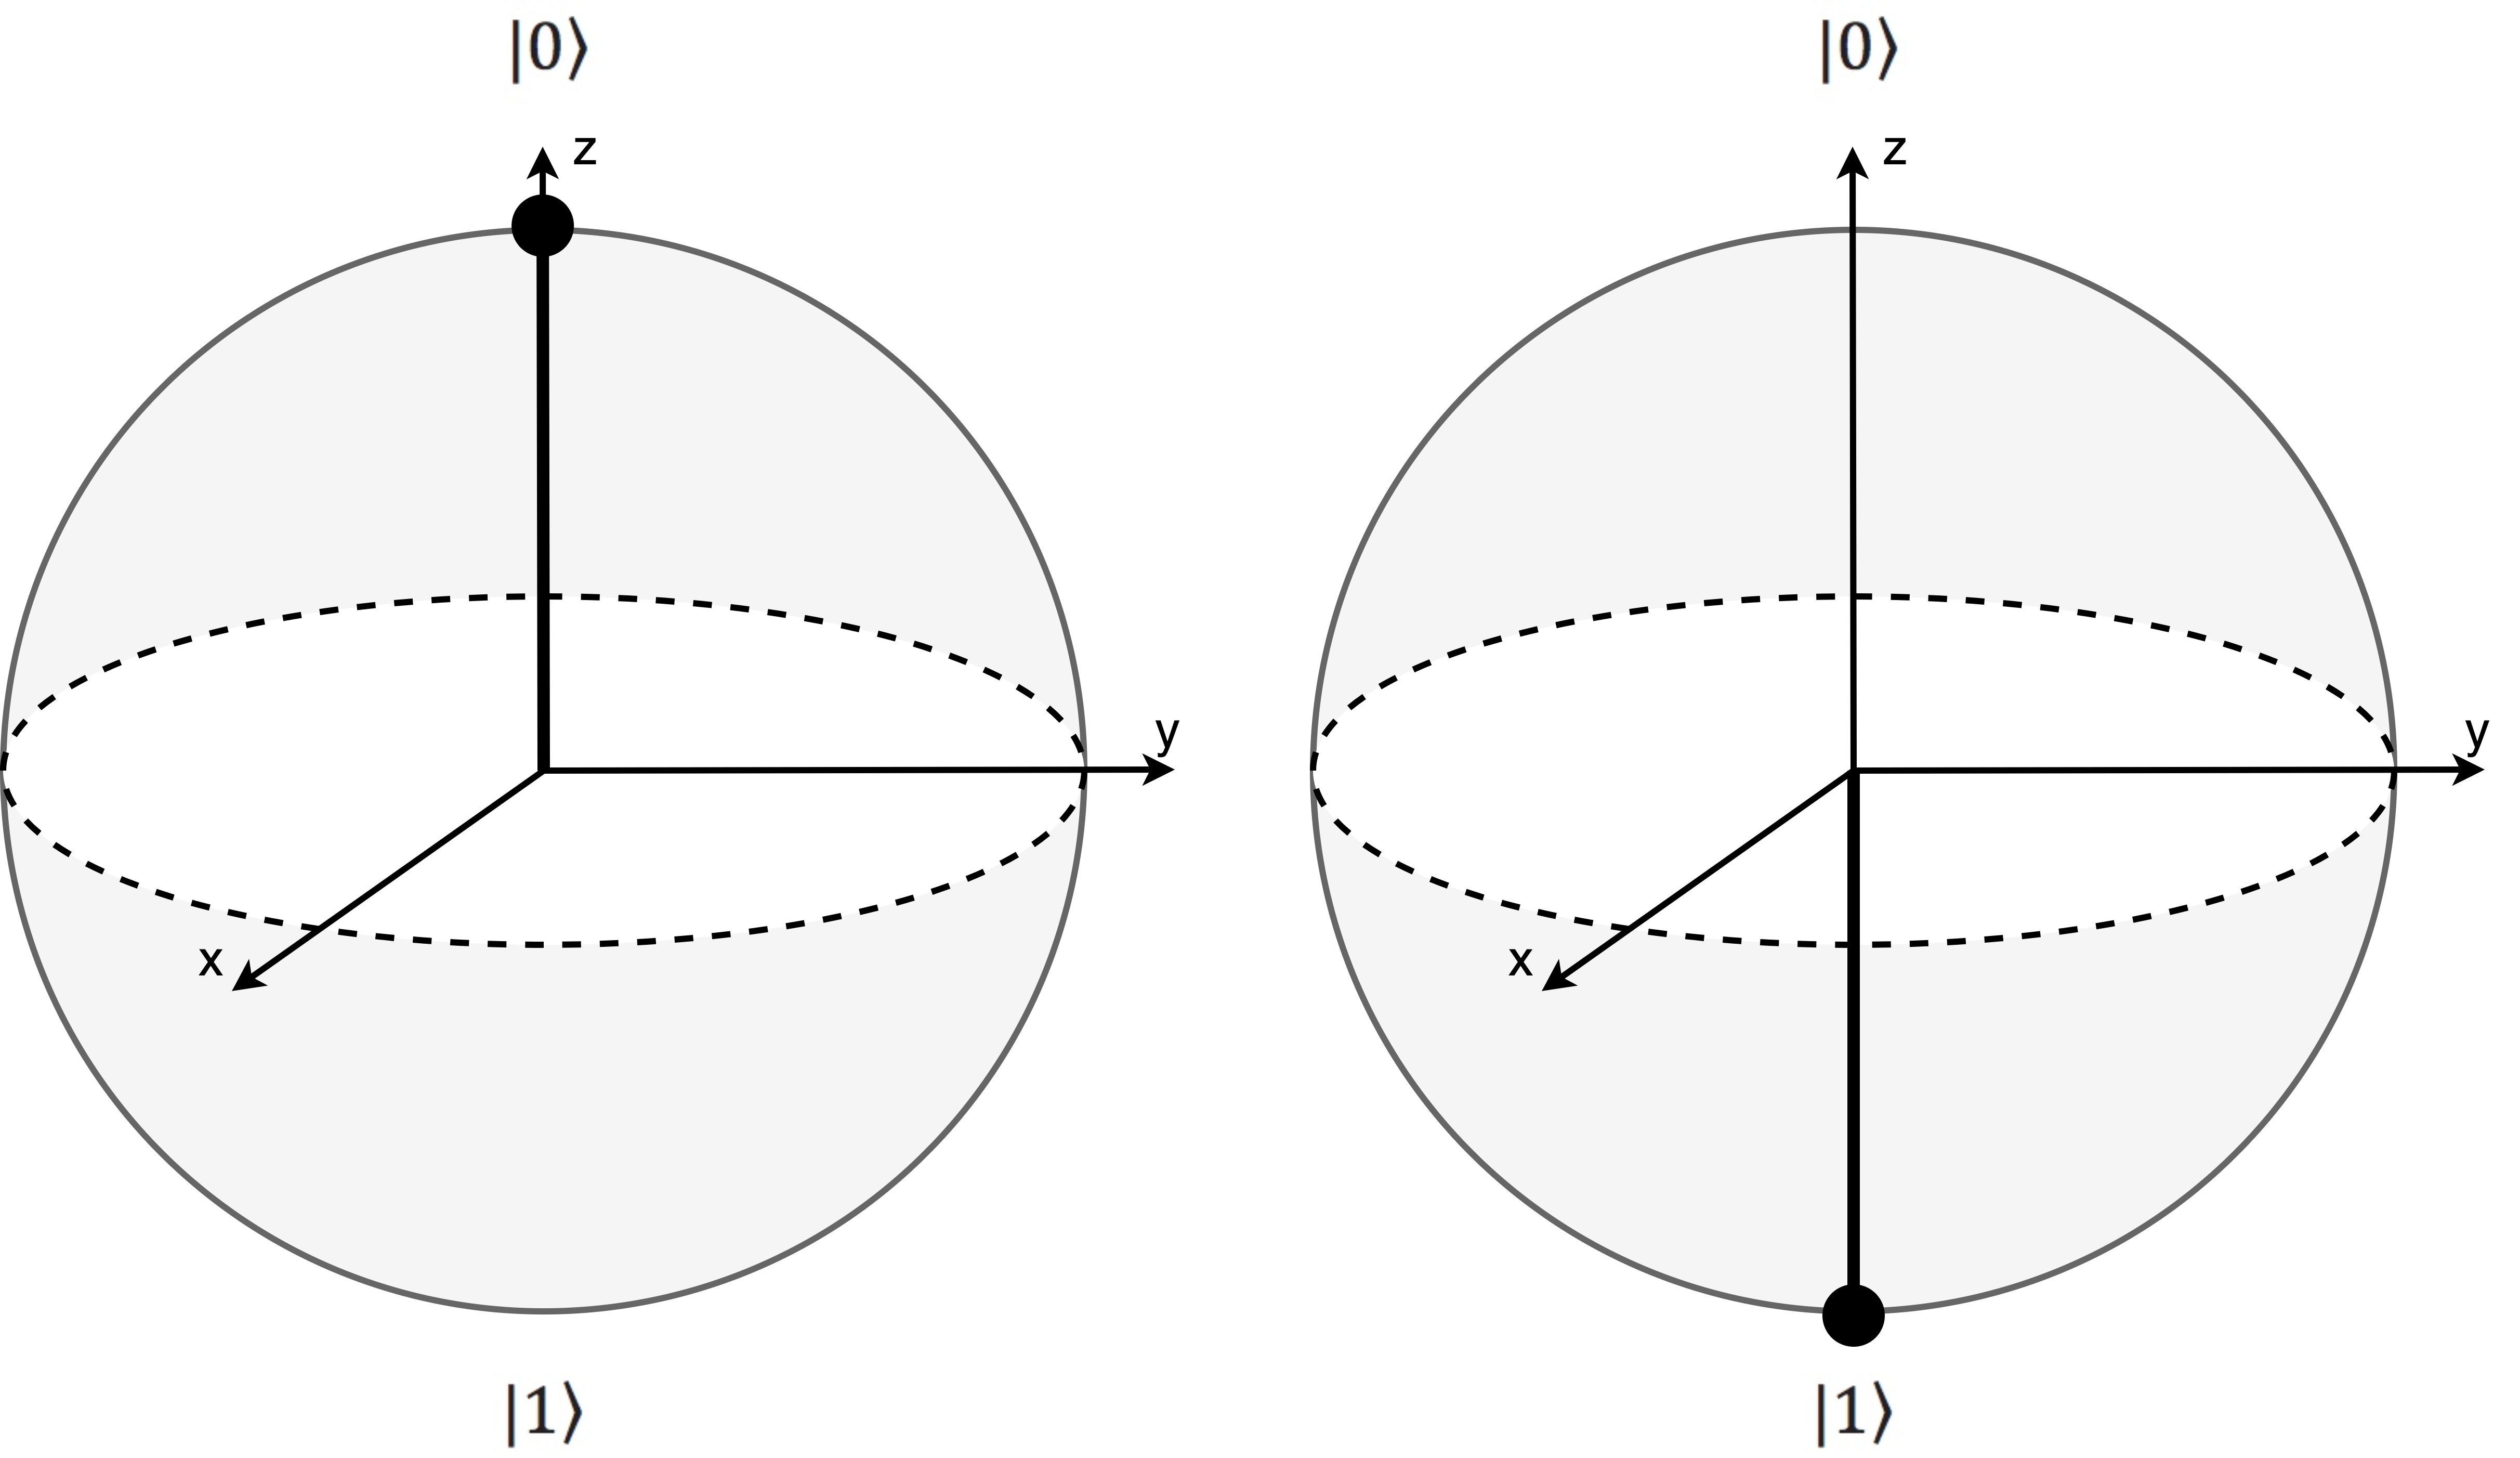
\includegraphics[width=.45\textwidth]{fig/bloch.png}
% \caption{A typical figure}
% \label{fig:exampleFig}
% \end{figure}


% \section{Images}

% All images and illustrations can be in color, but they must be visible in black-and-white, or gray tones.
% The image resolution on paper should be about 600 dpi for black-and-white images, and 150--200 dpi for grayscale images.

\bibliographystyle{unsrt}
\bibliography{example}

\end{document}

